\section{Überblick der wichtigsten Programmteile} % (fold)
\label{sec:überblick_der_wichtigsten_programmteile}

Im Folgenden wird auf die wichtigsten Teile des Programms nochmal genauer eingegangen und einzelne relevante Algorithmen und Datenstrukturen beschrieben und reflektiert.

\subsection{Model} % (fold)
\label{sub:model}
Das Model teilt sich in drei Hauptkomponenten auf: Die Spielerverwaltung (Leben und Geld) im Paket \class{model.player}, die Levelverwaltung (Zeitlicher Ablauf der Wellen) im Paket \class{model.level} und die Welt an sich im Paket \class{model.maze} mit Kreaturen und Türmen. Das \class{PlayerModelInterface} und die implementierende Klasse \class{Player} sind sehr einfach (eigentlich nur Resourcen erhöhen / verringern) und werden daher nicht genauer betrachtet. Auf die anderen beiden Teile wird dagegen im Folgenden noch genauer eingegangen, wobei die Welt aufgrund der Komplexität noch weiter unterteilt wird. Grundlegend für beide sind Aktionen, die zunächst kurz erklärt werden.

\subsubsection{Akteure und Aktionen} % (fold)
\label{ssub:aktionen}
Alle Objekte, die im Rahmen der Spielzeit agieren, implementieren das \class{ActorInterface} -- ein Funktionales Interface, das nur eine Methode \class{void act(double dt)} beinhaltet. Alle Akteure können beliebig auf das Fortschreiten der GameZeit reagieren. Häufig ist die Entscheidung, was als nächstes getan wird, jedoch nicht bei jedem Tick zu treffen, sondern kann in eine gewisse Spanne andaurnde Aktionen untergliedert werden. Die Klasse \class{Action} bietet eine abstrakte Implementierung eines Akteurs, der solange eine bestimmte Aktion durchführt, bis eine Abbruchbedingung erfüllt ist. Konkrete Implementierungen davon sind \class{CountdownAction}, die als Abbruchbedingung das Ablaufen einer Zeitspanne hat, sowie \class{MoveAction}, die als Abbruchbedingung das Erreichen eines gewissen Punktes oder beweglichen Objektes hat. Diese Klassen bieten die Grundlage für alle wiederholenden Aktionen.
% subsubsection aktionen (end)
\subsubsection{Das Paket level} % (fold)

\label{ssub:level}

Die Aufgabe des Level Pakets ist wie gesagt die zeitliche Steuerung der Creep-Wellen. Sie bietet nach außen für die View ein Binding, wie viel Prozent des Spiels schon vergangen sind. Nach einem gewissen Countdown erstellt sie -- entsprechend der Konfiguration des aktuellen Levels -- eine Liste von Kreaturen in der \class{CreatureFactory} und beauftragt das \class{MazeModelInterface} diese in das Spiel einzufügen. Anschließend wird der Countdown neu gestartet.
% subsubsection level (end)

\missingfigure{Klassendiagramm Level}

\subsubsection{Das Paket maze -- Kreaturen} % (fold)
\label{ssub:maze_kreaturen}
Vieles zu den Kreaturen wurde bereits in den vorherigen Kapiteln (insb \ref{sub:strategy_pattern}) erklärt. Im Folgenden wird sich daher auf die Struktur fokusiert, die bisher noch nicht erwähnt wurde.

Es gibt verschiedene Kreaturenarten, die in einem Enum \class{CreatureType} spezifiziert sind. Dieses Enum enthält auch die Default-Werte der Typen für die Leben, Geschwindigkeit, Wert und Bewegungsalgorithmus. Ausgehend von diesen Default-Werten werden die Creeps in der \class{CreatureFactory} mit einem bestimmten Zeitfaktor abgewandelt (Kreaturen werden mit der Zeit stärker, geben aber auch etwas mehr Geld).

\begin{lstlisting}[language=Java]
public enum CreatureType {
  DUMB(3, 10, 1, new RandomMovement()),
  NORMAL(1, 10, 1, new NoSightMovement()),
  TOUGH(0.8, 30, 3, new NoSightMovement());
  //... Attribute mit Gettern
  private CreatureType(double defaultVelocity, int defaultLifes,
   int defaultValue, MovementInterface defaultMovement) {
   //... Zuweisung
  }
}
\end{lstlisting}

Die Kreaturen sind Akteure und werden daher von der GameLoop aktualisiert. Sie besitzen eine aktuelle \class{Action}, die z.B. eine \class{MoveAction} zu einem bestimmten Ziel ist. Ist dieses Ziel erreicht, sucht die Kreatur mit dem gesetzten Bewegungsalgorithmus das nächste Ziel und erstellt dafür eine neue MoveAction. Zusätzlich wird bei jeder Positionsänderung überprüft, ob Kreaturen in der Reichweite sind, die andere Informationen über die Welt haben (\class{VisitedMap}). Falls das der Fall ist, wird die Bewegungsaktion durch eine \class{CountdownAction} vorübergehend unterbrechen, um sich mit der anderen Kreatur zu unterhalten. Danach wird die Bewegung fortgesetzt.

\paragraph{VisitedMap} Wie bereits in Kapitel~\ref{sub:neuer_ansatz_im_eigenen_projekt} erwähnt, ist die VisitedMap zentraler Bestandteil der scheinbaren Intelligenz der Kreaturen. Da diese sehr oft verglichen wird, war hier eine effiziente Implementierung notwendig. Die Speicherkomplexität der Map liegt in \(O (c\cdot n \cdot m)\), wobei \(c\) die Anzahl der Creeps, und \(n\times m\) die Abmessung der Welt ist (im aktuellen Spiel \(10\times20\)). Sind jedoch alle \(c\) Kreaturen nah zusammen, versucht jede Kreatur mit jeder anderen zu kommunizieren, also \(c\cdot (c-1)\) und jeder Vergleich der Arrays benötigt \(O(n\cdot m)\) Schritte \(O(c^2\cdot n\cdot m)\). Eine Optimierung gelingt dadurch, dass für die Arrays ein Hash-Wert erstellt wird und für den Vergleich herangezogen wird. Nur wenn die Hash-Werte unterschiedlich sind, wird über das gesamte zweidimensionale Array iteriert und die Informationen zusammengefügt. Dadurch muss in dem gleichen Fall nur eine Kreatur mit allen anderen den Zustand synchronisieren -- alle anderen Vergleiche sind unabhängig von der Spielfeldgröße \(\Rightarrow O(c\cdot n \cdot m + (c-1)\cdot(c-1)\cdot1) = O(c \dot n \cdot m + c^2) \). Da sich die Figuren in der Regel eine längere Zeit in der Gruppe bewegen, unterscheidet sich der State auch seltener, wodurch der Vorteil des Hashwertes noch deutlich wird. Nicht beachtet wurde dabei bisher die Komplexität zur Berechnung des Hash-Wertes. Zunächst wurde die Methode \class{Arrays.deepHashCode(Object[] a)} zur Berechnung verwendet, die allerdings in Benchmarks immer noch eine hohe Auslastung anzeigte. Stattdessen wurde anschließend das Zobrist Hashing \todo{Referenz} verwendet. Das ermöglichte, den Hash-Wert bei Änderungen direkt mit einer einfachen Bit-Operation anzupassen, statt ihn mit dem gesamten Array neu zu berechnen. Dies führte zu einem vernachlässigbaren Aufwand zur Hashberechnung und der Vergleich war effizient genug, dass dies kein Problem mehr darstellte. Die tatsächlich gemessenen Laufzeitergebnisse sind in Grafik~\ref{fig:benchmark} dargestellt.
\begin{figure}[tb]
	\centering
	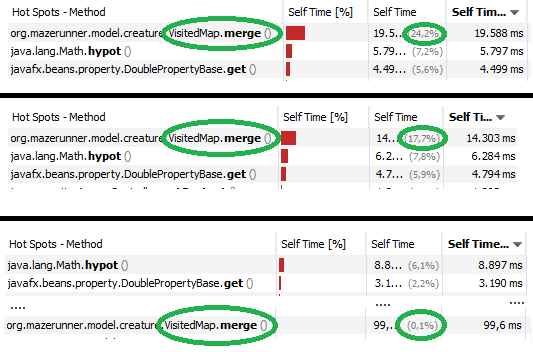
\includegraphics{images/benchmark.png}
	\caption{Laufzeitanalyse der drei Implementierungen der Merge-Methode. Die Daten wurden mit Java Visual VM aufgenommen und zeigen einen Ausschnitt der rechenintensivsten Methoden gemessen zur Laufzeit mit 600 Kreaturen und dem gleichen Labyrinth Setup. Die erste Tabelle zeigt die Laufzeit ohne Hashing, die zweite mit \lstinline{Arrays.deepHashCode}, die dritte die letztliche Programmierung mit Zobrist Hashing.}
	\label{fig:benchmark}
\end{figure}
% subsubsection maze_kreaturen (end)
% subsection model (end)
% section überblick_der_wichtigsten_programmteile (end)